\chapter{Analysis of Resource Optimized FFT}\label{Chapter4}
From the analysis given in chapter \ref{Chapter3}, it was found that FFT is the most computationally intense algorithm of FHEW library, and optimization related to converting the FFT from double precision to single precision is not supported  because of the limitations as discussed in section \ref{3.10}. The idea is to implement the algorithm on hardware and to achieve better efficiency by parallelising the application by simultaneously running multiple FFT's in parallel. However this is possible only if there are sufficient resources available on hardware to support it. The rationale behind this chapter is to analyze a double precision resource optimized 1024-point FFT such that the resources consumed are very less so that the achievable parallelism can be estimated.

\noindent The tool used for the analysis is Vivado HLS. The technique used is the bottom-up analysis of the FFT i.e. implementing the smallest FFT computation unit and scaling it up to yield a 1024 point FFT such that the accuracy is not compromised and also the resources are optimized. 
\section{A Brief about Vivado HLS}
It is a high level synthesis tool which allows to create IP's from a C, C++, System C specification and it automatically generates RTL. It supports various data types integer, floating and double which is the primary requirement for writing the specification for FFT based on our requirement. It provides various optimization directives, which help in improving the performance of an algorithm by controlling the synthesis process. It provides generation of an IP core of an application, which in turn helps in accelerating the computationally intense parts of the application on programmable logic part of the hardware e.g. FPGA's. It also supports choice of hardware so that the performance can be analyzed thoroughly in terms of area and latency parameters for different implementations or on different hardware. 

In this chapter, an analysis of resource optimized 1024 point double precision FFT is performed starting from a single butterfly structure i.e. Radix 2 FFT, as described in figure \ref{fig:butterfly}. A C specification is written supporting the implementation of butterfly structure which later is scaled up to compute a 1024 point FFT, by limiting the resources with the help of various resource optimization directives provided by HLS and performing design space exploration.

\section{A Brief about FFT Algorithm}
FFT is an algorithm which allows efficient computation of discrete fourier transform by limiting the number of computations used for computing the DFT.

\vspace{0.25cm}
The DFT of a signal x[n] is given by the expression:

\hspace{3cm} $X(e^{jw}) =\sum_{n=0}^{N-1} x[n]\cdot e^{-jwn}$ \hfill eqn[4.1]

\vspace{0.25cm}
For a finite duration signal, DFT is defined as: 

\hspace{3cm} $X(e^{jw}) = \sum_{n=0}^{N-1} x[n]\cdot e^{-j(2\times \pi\times k/N)n}$ \hfill eqn[4.2] 

\vspace{0.25cm}
Given $W\textsubscript{N} =e^{-j(2\times \pi/N)}$, the above expression can be rewritten as:

\hspace{3cm} $X(e^{jw}) = \sum_{n=0}^{N-1} x[n]\cdot W\textsubscript{N}^{kn}$ \hfill eqn[4.3]

\vspace{0.25cm}
\noindent Referring equation 4.3, it can be seen that the expression requires N(N-1) complex additions and $N^{2}$ complex multiplications to compute a complex N point DFT.
\noindent The fast fourier transform is derived from DFT by separating the even and odd indexes of the summation. It computes the DFT by using a reduced number of computations by exploring the symmetry of the term $W\textsubscript{N}$ which is called the twiddle factor. The various properties of $W\textsubscript{N}$ are:
\begin{itemize}
    \item 
    $W\textsubscript{N}^{N}=1$
        \item 
        It is periodic with N. i.e. 
        $W\textsubscript{N}^{N} = W\textsubscript{N}^{N+kN}$
        \item
  It is symmetric. i.e. $W\textsubscript{N}^{k+N/2}= -W\textsubscript{N}^{k}$
\end{itemize}
By exploring the symmetries given above, the number of computations are reduced in a way such that lesser number of twiddle factors is required to be computed. 

\section {Analysis of Butterfly Structure}

The basic computation structure in FFT is the butterfly structure which computes the two point FFT. The structure takes  two complex numbers a and b as input and produces two complex numbers A and B as output such that,

\hspace{3cm} $A=a+W\textsubscript{N}\cdot b$

\hspace{3cm} $B=a-W\textsubscript{N}\cdot b$

\noindent as shown in figure \ref{fig:butterfly}.
%figure
\begin{figure}[H]
\centering
\includegraphics[scale=0.75]{figures/butterfly.png}
\caption{Basic Butterfly Structure for FFT Computation}
\label{fig:butterfly}
\end{figure}


\noindent The C function for the implementation of the butterfly structure is defined in listing \ref{listing:2}.

\lstset { %
	language=C,
	backgroundcolor=\color{lightgray}, % set backgroundcolor
	%basicstyle=\footnotesize,% basic font setting
	basicstyle=\ttfamily\scriptsize,
	%\basicstyle=\ttfamily\scriptsize,
	keywordstyle=\color{blue}\ttfamily,
	stringstyle=\color{red}\ttfamily,
	commentstyle=\color{darkgray}\ttfamily,
	breaklines=true	
}
\lstset{framesep=-10pt, xleftmargin=-10pt}
\begin{lstlisting}[caption={Sample Code to Implement Butterfly Structure},label={listing:2}]
void butterfly(double X_R[2],double X_I[2],double w_re, double w_im)
{   
    //declare temporary variables
    double E1R, E1I, E2R, E2I;
    
    E1R = X_R[0], E2R = X_R[1];
    E1I = X_I[0], E2I = X_I[1];
    
    //computes the First index output
    X_R[0]=E1R + E2R;
    X_I[0]=E1I + E2I;
    
    //computes the second index output
    X_R[1] = (E1R-E2R)*w_re - (E1I-E2I)*w_im;
    X_I[1] = (E1R-E2R)*w_im + (E1I-E2I)*w_re;
}
\end{lstlisting}



The C implementation is verified for functionality by testing with a C test bench, and synthesized for ZC7020 zedboard. The synthesis report was studied and it was found that the computation takes 18 cycles to finish the execution. The utilization aspects specified that it uses 4 instances of double precision multiplier, 2 instances of double precision subtractor unit, one instance each of double precision adder and double precision adder-subtractor unit which counts for about 25 percent DSP units utilization for only one butterfly unit computation. 
\subsection{Area Optimization}\label{4.3.1}
On thorough analysis of the butterfly unit it can be seen that the four multiplications can be performed by using only one double precision multiplier and addition and subtraction can be performed by the same adder-subtractor unit, if a few cycles of latency are compromised. The system is optimized by applying the directives to bind the resources to various operators. The following optimizations are applied to the code:
\begin{itemize}
\item
\textbf{ALLOCATION:} The allocation directive is used to specify the limit on the DSP cores to be used in the algorithm to implement resource sharing at the expense of latency. It can be specified as:

\# pragma HLS ALLOCATION instances=dmul limit=1 operation

\noindent This limits the number of double precision multipliers to 1.
\item
\textbf{RESOURCE:} The resource directive is used to specify that the computation of a specific variable will be executed by which DSP core. It can be implemented as:

\# pragma HLS RESOURCE variable=temp core=dAddSub\_fulldsp

\noindent This specifies that the temp variables operation should be computed by double precision adder-subtractor unit.

\noindent It should be noted the RESOURCE directive works only for the first assignment of a variable. If a variable is reassigned multiple times in a specification, the directive will work only for the first assignment. Different temporary variables should be defined to optimize further the reassignments of a variable.

In the above implementation of butterfly unit, the computation of X\_R[0], X\_I[0], X\_R[1] and X\_I[1] are mapped to be computed by adder-subtractor unit.
\item
\textbf{CONFIG BIND:} It is a GUI directive. It helps to minimize the number of operations used. It can be specified from Vivado GUI, by navigating through solution settings as specified below:

Solution-\textgreater Solution\_Settings-\textgreater Add-\textgreater config\_bind.

Figure \ref{fig:configbind} demonstrates the usage of config bind directive.

\begin{figure}[H]
\centering
\includegraphics[scale=0.5]{figures/config_bind.png}
\caption{Config Bind Directive}
\label{fig:configbind}
\end{figure}

The config bind directive is used to minimize the operations for double precision subtractor in the above FFT butterfly unit implementation.
\end{itemize}
\subsection{Comparison of Results}
The implementation of butterfly unit, was executed with the application of different optimization directives as given in section \ref{4.3.1}. The trade-off between the computation time and the resource utilization can be easily observed from the area vs. latency curve as given in figure \ref{plot_butterfly}.

 \begin{figure}[H]
\centering
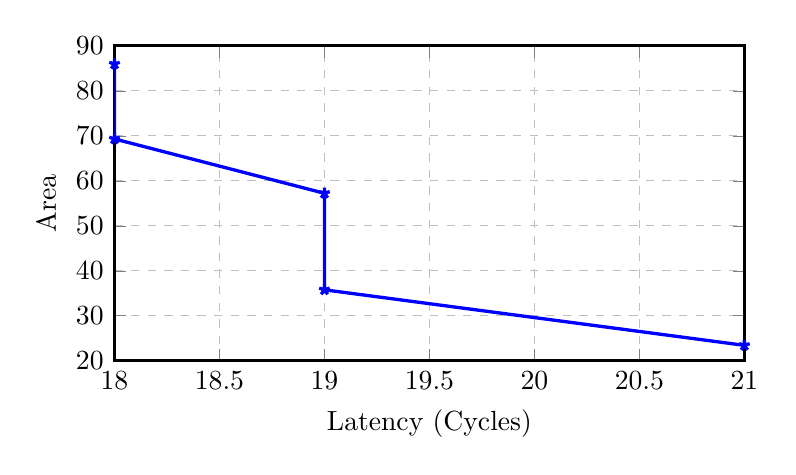
\begin{tikzpicture}
\begin{axis}[
scale only axis,
height=4cm,
width=8cm,
    xlabel={Latency (Cycles)},
    ylabel={Area},
    xmin=18, xmax=21,
    ymin=20, ymax=90,
    xtick={18,18.5,19,19.5,20,20.5,21},
    ytick={20,30,40,50,60,70,80,90},
    legend pos=north east,
    ymajorgrids=true,
    xmajorgrids=true,
    grid style=dashed,
    very thick
]
\addplot[
    color=blue,
    mark=star,
    %smooth
    ]
    coordinates {
    (18,85.95)(18,69.3)(19,57.225)(19,35.77)(21,23.429)
    };
\end{axis}
\end{tikzpicture}
\caption{Area Vs. Latency Curve for Butterfly Unit Implementation}
\label{plot_butterfly}
\end{figure}

From the graph, it can be seen that the latency value of 21 yields the minimum area. This value corresponds to the optimization, which limits the resources to one double precision adder subtractor unit and one double precision multiplier unit as given in table \ref{Table 4.1}. 

The results of design space exploration with the application of area optimization directives were compared against the results of the implementation with no optimization. The comparison is also given in table \ref{Table 4.1}.
\begin{table}[H]
\centering
\caption{Synthesis Results Comparison for Design Space Exploration for Butterfly Unit Execution for Resource Optimization for Zedboard ZC702}
\label{Table 4.1}
\begin{tabular}{||m{3cm}|m{2cm}|m{2cm}|m{2cm}|m{2cm}|m{2cm}||}
\hline
Metric & No Optimization & Resource Directive& Allocation Directive (3 Multipliers) & Allocation Directive (2 Multipliers) & Area Optimized  \\
\hline
\multicolumn{6}{||c||}{Timing Estimates}\\
\hline
Latency(Cycles) & 18 &18&19&19& 21\\
\hline
\multicolumn{6}{||c||}{Area Estimates}\\
\hline
Number of Multipliers & 4 & 4&3&2& 1\\
\hline
Number of Subtractors & 2 & 1&1&0&0\\
\hline
Number of Adders & 1 & 1&1&0&0\\
\hline
Number of Add-Sub Units & 1 & 0&0&1&1\\
\hline
DSP48E (\%age Utilization) & 25 & 22&17&11&6\\
\hline
LUT's (\%age Utilization) &13 & 8&8&4&4\\
\hline
Flip Flops (\%age Utilization) & 3 & 2&2&1&1\\
\hline
\end{tabular}

\end{table}

From table \ref{Table 4.1}, it can be seen that the resources are reduced by a significant factor i.e. the implementation is limited to use only one double precision multiplier and only one double precision adder-subtractor unit which is the minimum requirement for performing the calculations. However 3 cycles of latency are compromised. 

The resource utilization could be even lesser, if floating point data types are used e.g. the double precision multiplier uses 1149 LUT's to implement an adder unit, whereas the single precision floating point uses 390 LUT's to implement an adder unit.

\section {Analysis of 1024-Point FFT}\label {4.4}
The above implementation of butterfly unit is scaled up to compute a 1024 point FFT. The twiddle factors for computing the FFT are pre computed and supplied as array variables which are stored in BRAM to save the processing power at runtime. At a time two input samples are packed and sent to call the butterfly module which is already optimized by limiting the number of resources. Computation of N point FFT requires log\textsubscript{2}N stages, each computing N/2 butterfly operations.

The performance is further enhanced by exploring other pragmas available in Vivado HLS. e.g.
\begin{itemize}
\item
INLINE: This is used to replace function calls with function definitions. It is implemented by placing

\hspace{3cm}\# pragma HLS INLINE

at the beginning of the function body.
For computation of FFT the butterfly module is called several times, so it declared as INLINE using the above directive, to reduce the overhead of calling the functions.
\item
PIPELINE: This is used to use all resources concurrently in the algorithm. It is implemented by placing

\hspace{3cm}\# pragma HLS PIPELINE

\item
UNROLL: This is used to create multiple independent iterations of a loop simultaneously at the expense of resources. It is implemented by placing

\hspace{3cm}\# pragma HLS UNROLL \textit{unroll factor}

at the beginning of the loop body.
It should be noted the unroll factor must be provided otherwise the loop fails to unroll.
\end{itemize}

\noindent The design space exploration was performed for the FFT code with the application of different optimization pragmas as given in section \ref{4.4} and \ref{4.3.1}.

\noindent The performance analysis of the results of intermediate experiments of scaling the butterfly unit implementation to 1024 point FFT, which involves scaling the butterfly unit to first implement a 4-point FFT and then further scaling up to 16-point FFT and so on, is given as the area vs. latency curves as given in figure \ref {plot_4fft} to figure \ref{plot_128fft}.

The details of the design space exploration for the intermediate experiments is given in detail in tables \ref{4-point} to \ref{128-point}.


\begin{figure}[H]
\centering
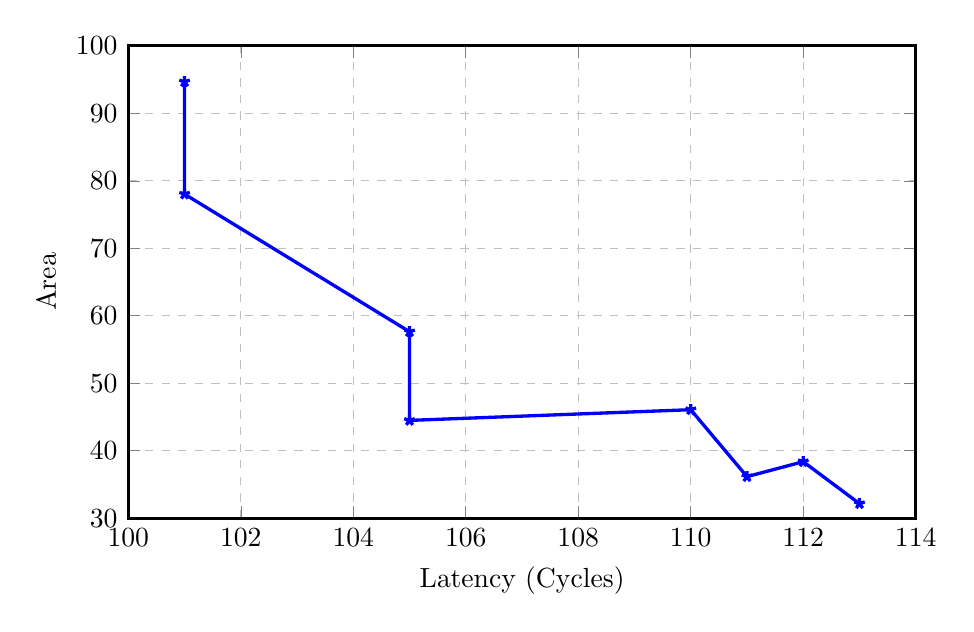
\begin{tikzpicture}
\begin{axis}[
scale only axis,
height=6cm,
width=10cm,
    xlabel={Latency (Cycles)},
    ylabel={Area},
    xmin=100, xmax=114,
    ymin=30, ymax=100,
    xtick={100,102,104,106,108,110,112,114},
    ytick={30,40,50,60,70,80,90,100},
    legend pos=north east,
    ymajorgrids=true,
    xmajorgrids=true,
    grid style=dashed,
    very thick
]
\addplot[
    color=blue,
    mark=star,
   % smooth
    ]
    coordinates {
    (101,94.675)(101,78.025)(105,57.6375)(105,44.495)(110,46.08)(111,36.165)(112,38.375)(113,32.166)
    };
\end{axis}
\end{tikzpicture}
\caption{Area Vs. Latency Curve for 4-Point FFT Implementation}
\label{plot_4fft}
\end{figure}
\begin{table}[H]
\centering
\caption{ Design Space Exploration Results for 4-Point FFT Computation for Zedboard ZC702}
\label{4-point}
\begin{tabular}{||m{1.5cm}|m{1.5cm}|m{1.5cm}|m{1.6cm}|m{1.6cm}|m{1.6cm}|m{1.4cm}|m{1.4cm}|m{1.4cm}||}
\hline
Metric & No Optimization & Resource & Allocation (3 Multipliers) & Allocation (2 Multipliers) & Allocation (1 multiplier) & Loop-1 Unroll (factor 2) & Loop 2-Unroll (factor 2) & Loop 1,2 Unroll (factor 2-2) \\
\hline
\multicolumn{9}{||c||}{Timing Estimates}\\
\hline
Latency (Cycles) & 101 & 101 & 105 & 105 & 113  & 112 & 111 & 110\\
\hline
\multicolumn{9}{||c||}{Area Estimates}\\
\hline
DSP48E  & 57 & 51 & 37 & 26 & 15 & 18 & 15 & 18\\
\hline
LUT's  &9042 & 6486 & 4953 & 4439 & 4120 &4890 & 5080 & 6740 \\
%\hline
%FF's & 4398 &3636 & 2822 & 2516 & 2137  &2287 & 2321 & 2647\\
\hline
\end{tabular}

\end{table}



\begin{figure}[H]
\centering
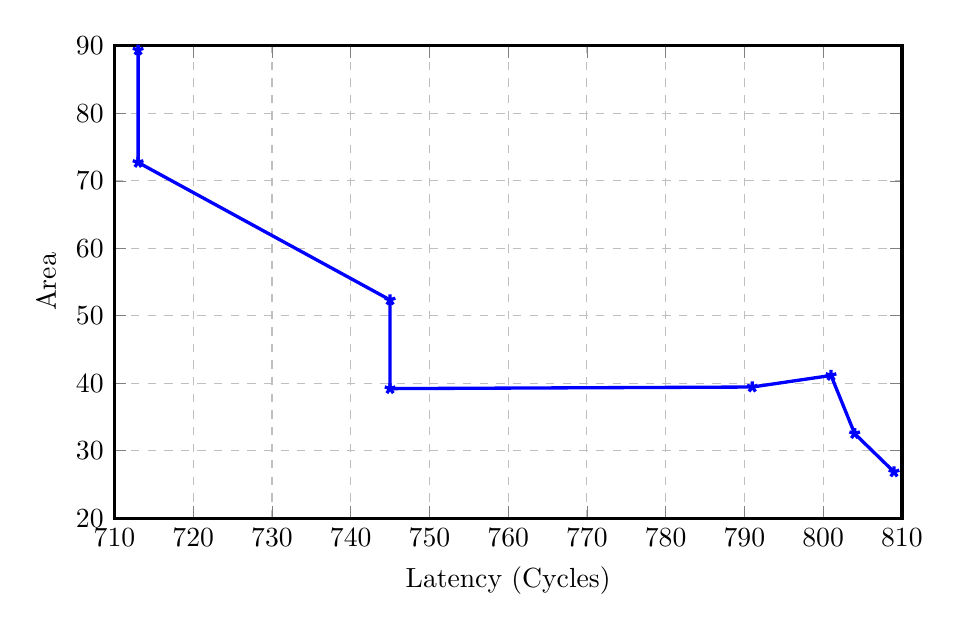
\begin{tikzpicture}
\begin{axis}[
scale only axis,
height=6cm,
width=10cm,
    xlabel={Latency (Cycles)},
    ylabel={Area},
    xmin=710, xmax=810,
    ymin=20, ymax=90,
    xtick={710,720,730,740,750,760,770,780,790,800,810},
    ytick={20,30,40,50,60,70,80,90},
    legend pos=north east,
    ymajorgrids=true,
    xmajorgrids=true,
    grid style=dashed,
    very thick
]
\addplot[
    color=blue,
    mark=star,
   % smooth
    ]
    coordinates {
    (713,89.37)(713,72.72)(745,52.345)(745,39.204)(791,39.441)(801,41.154)(804,32.54)(809,26.8625)
    };
\end{axis}
\end{tikzpicture}
\caption{Area Vs. Latency Curve for 16-Point FFT Implementation}
\label{plot_16fft}
\end{figure}
\begin{table}[H]
\centering
\caption{Design Space Exploration Results for 16-Point FFT Computation for Zedboard ZC702}
\label{16-point}
\begin{tabular}{||m{1.5cm}|m{1.5cm}|m{1.5cm}|m{1.6cm}|m{1.6cm}|m{1.6cm}|m{1.4cm}|m{1.4cm}|m{1.4cm}||}
\hline
Metric & No Optimization & Resource & Allocation (3 Multipliers) & Allocation (2 Multipliers) & Allocation (1 multiplier) & Loop-1 Unroll (factor 2) & Loop 1-Unroll (factor 4) & Loop 1,2 Unroll (factor 2-2) \\
\hline
\multicolumn{9}{||c||}{Timing Estimates}\\
\hline
Latency (Cycles) & 713 &713 &745 &745 & 809 & 804 & 801 & 791\\
\hline
\multicolumn{9}{||c||}{Area Estimates}\\
\hline
DSP48E  & 57 & 51 &37 & 26 &  15 & 18 & 22 & 18\\
\hline
LUT's  &7769 & 5213 & 3683 & 3169 & 2847 & 3490 & 4597 & 5146\\
%\hline
%FF's & 4199 & 3437 & 2612 & 2295 &  1916 & 2187 & 2622 & 2940\\
\hline
\end{tabular}

\end{table}

\begin{figure}[!h]
\centering
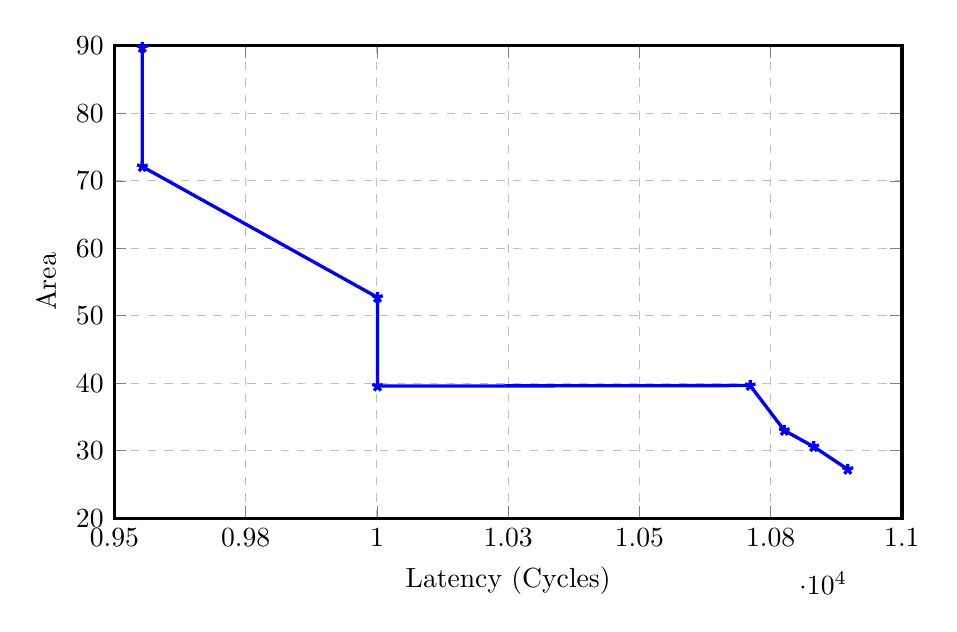
\begin{tikzpicture}
\begin{axis}[
scale only axis,
height=6cm,
width=10cm,
    xlabel={Latency (Cycles)},
    ylabel={Area},
    xmin=9500, xmax=11000,
    ymin=20, ymax=90,
    xtick={9500,9750,10000,10250,10500,10750,11000},
    ytick={20,30,40,50,60,70,80,90},
    legend pos=north east,
    ymajorgrids=true,
    xmajorgrids=true,
    grid style=dashed,
    very thick
]
\addplot[
    color=blue,
    mark=star,
   % smooth
    ]
    coordinates {
    (9553,89.745)(9553,72.098)(10001,52.720)(10001,39.579)(10711,39.658)(10776,33.004)(10832,30.595)(10897,27.2395)
    };
\end{axis}
\end{tikzpicture}
\caption{Area Vs. Latency Curve for 128-Point FFT Implementation}
\label{plot_128fft}
\end{figure}
\begin{table}[H]
\centering
\caption{Design Space Exploration Results for 128-Point FFT Computation for Zedboard ZC702}
\label{128-point}
\begin{tabular}{||m{1.5cm}|m{1.5cm}|m{1.5cm}|m{1.6cm}|m{1.6cm}|m{1.6cm}|m{1.4cm}|m{1.4cm}|m{1.4cm}||}
\hline
Metric & No Optimization & Resource & Allocation (3 Multipliers) & Allocation (2 Multipliers) & Allocation (1 multiplier) & Loop-1 Unroll (factor 2) & Loop 2-Unroll factor (2) & Loop 1,2 Unroll (factor 2-2) \\
\hline
\multicolumn{9}{||c||}{Timing Estimates}\\
\hline
Latency (Cycles) & 9553 & 9553 & 10001 &10001 & 10897 & 10776 &  10832 & 10711\\
\hline
\multicolumn{9}{||c||}{Area Estimates}\\
\hline
DSP48E  & 57 & 51 & 37 & 26 & 15 & 18 & 15 & 18\\
\hline
LUT's  &  7859 & 5303 & 3773 & 3259 & 2937 & 3603 & 3743 & 5198\\
%\hline
% FF's &  4145 & 3383 & 2558 & 2241 & 1862 & 2154 & 2183 & 2773\\

\hline
\end{tabular}

\end{table}





\noindent The utilization estimates by scaling the resource optimized butterfly for computing 1024 Point FFT are given in detail in table \ref{Table 4.3}.

\begin{table}[!h]
\centering
\caption{Synthesis Results Comparison for Resource Optimized 1024 Point FFT for Performance Optimization for Zedboard ZC702}
\label{Table 4.2}
\begin{tabular}{||m{4cm}|m{2.5cm}|m{2.5cm}|m{2.5cm}|m{2.5cm}||}
\hline
Metric & Area Optimized & INLINE & Pipeline & Unroll (Factor 8)\\
\hline
\multicolumn{5}{||c||}{Timing Estimates}\\
\hline
Clock (ns)&8.23 &8.23&8.23& 9.57\\
\hline
Latency(Cycles) &118805 & 118805 &119828 &126754\\
\hline
\multicolumn{5}{||c||}{Area Estimates}\\
\hline
DSP48E & 15& 15 &15 & 30 \\
\hline
LUT's & 3035 & 3035 &2909 &51644\\
\hline
Flip Flops & 1923 & 1923 & 2052 &16973\\
\hline	
\multicolumn{5}{||c||}{Profiling}\\
\hline
Time To compute FFT &1.19ms&1.19ms&1.2ms&1.27ms\\
\hline
\end{tabular}

\end{table}

The corresponding area vs. latency curve is given as:  \begin{figure}[!h]
\centering
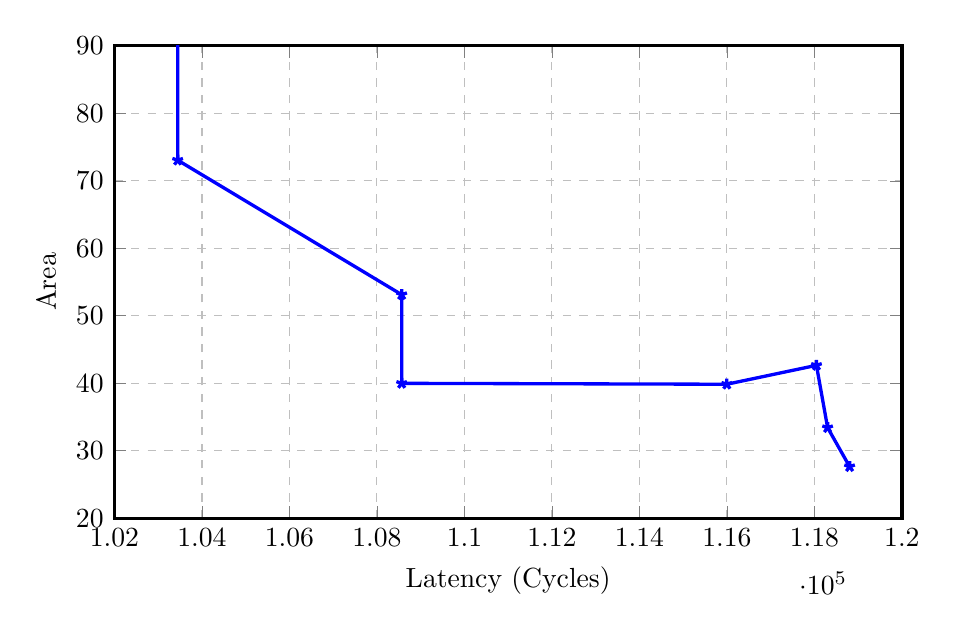
\begin{tikzpicture}
\begin{axis}[
scale only axis,
height=6cm,
width=10cm,
    xlabel={Latency (Cycles)},
    ylabel={Area},
    xmin=102000, xmax=120000,
    ymin=20, ymax=90,
    xtick={102000,104000,106000,108000,110000,112000,114000,116000,118000,120000},
    ytick={20,30,40,50,60,70,80,90},
    legend pos=north east,
    ymajorgrids=true,
    xmajorgrids=true,
    grid style=dashed,
    very thick
]
\addplot[
    color=blue,
    mark=star,
   % smooth
    ]
    coordinates {
    (103445,90.154)(103445,73.054)(108565,53.129)(108565,39.9875)(115998,39.854)(118047,42.654)(118302,33.425)(118805,27.646)
    };
\end{axis}
\end{tikzpicture}
\caption{Area Vs. Latency Curve for 1024-Point FFT Implementation}
\label{plot_1024fft}
\end{figure}

\noindent It should be noted that for computation of 1024 Point FFT:
\begin{itemize}
\item
The loops for execution of successive butterfly units are pipelined but it results in increase in the minimum clock period. 
\item
The loops used to compute FFT are unrolled by a factor of 8 which in turn ends up using almost 90 percent resources on Z702 zedboard as per the analysis in Vivado HLS. However only a few cycles of latency are saved. If more resources can be supplied, by changing hardware, more unroll options can be explored. 
\end{itemize}


All the above implementations use only one double precision multiplier and only one double precision adder-subtractor unit. Additions and subtractions are performed by the same adder-subtractor unit. 
From table \ref{Table 4.2}, if the time to compute 1024 Point FFT is computed it can be seen that it takes minimum as 1.19ms sec by the area optimized FFT. The unroll by a factor of 8 consumes almost 97 percent of LUT's for Zedboard(ZC702). To explore further parallelism we might need to use other hardware which supplies more number of resources. 

%\section{Performance Analysis by changing the Underlying Hardware}
%The given area optimization's are applied to Virtex VC709 board for the same algorithm and the results were compared in terms of resource consumption, latency and time taken to compute the 1024 point FFT. The comparison is as described in table \ref{Table 4.3}.

%The choice of platform depends on a lot of factors e.g. cost, area, performance requirements, e.g. If a latency optimized designed is required, parallelism should be exploited at the expense of resources, as the total number of resources are more. 

For efficient implementation of FHEW on hardware, the area optimized FFT algorithm can be used as a packaged core and can be used to provide executions of several FFT's running in parallel to increase the speed of algorithm. 

%\begin{table}[!h]
\centering
\begin{tabular}{||m{5.5cm}|m{4cm}|m{4cm}||}
\hline
Metric & Virtex (VC709) & Zedboard (ZC702)  \\
\hline
\multicolumn{3}{||c||}{Timing Estimates}\\
\hline
Estimated Clock (ns) & 9.83 & 8.23\\
\hline
Latency (Cycles) &98325&118805\\
\hline
\multicolumn{3}{||c||}{Area Estimates}\\\cline{1-3}

DSP48E & 15 & 15\\
\hline
LUT's &2238 & 3035\\
\hline
Flip Flops  &1862 & 1923\\
\hline
\multicolumn{3}{||c||}{Profiling}\\
\hline
Time To compute FFT &98.3us& 1.19ms\\
\hline
\end{tabular}
\caption{Performance Comparison of Double Precision Area optimized FFT on VC709 and ZC702 board}
\label{Table 4.3}
\end{table}

In the next chapter another computationally intensive algorithm, deep neural network is explored for modification in arithmetic from floating point to fixed point.




